%!TEX encoding = UTF-8 Unicode
\documentclass{ctexart}
\usepackage{color}
\usepackage{xcolor}
\usepackage{amsmath}
\usepackage{amssymb}
\usepackage{esint}
\usepackage{graphicx}
\usepackage{bm}
\usepackage{multirow}

\numberwithin{equation}{section}

\newtheorem{Definition}{\hspace{2em}定义}
\newtheorem{theorem}{\hspace{2em}定理}
\newtheorem{lemma}{\hspace{2em}引理}
\newtheorem{Proof}{证明}
\newtheorem{remark}{注}
\newtheorem{example}{例子}

\colorlet{RED}{red}

\begin{document}

\title{大规模并行处理器编程-实践方法}

\author{杨丰}
\date{}
\maketitle

\tableofcontents

\newpage
\section*{推荐序}
Wen-mei 和 David 的《大规模并行处理器编程》(第四版)由两位杰出的计算机科学家和 GPU 计算先驱撰写,
作者为 Wen-mei W. Hwu、David B. Kirk 和 Izzat El Hajj,继续为该领域做出了宝贵贡献。 创建新的计算模型。

GPU 计算已成为现代科学的重要工具。 本书将教您如何使用该仪器,并为您提供解决最具挑战性问题的超强工具。 
GPU 计算将成为一台让您看到未来的时间机器,一艘带您前往触手可及的新世界的宇宙飞船。

解决世界上许多最具影响力的问题都需要计算性能。 从计算机历史的开始,架构师就寻求并行计算技术来提高性能。 
一百倍的提升相当于依赖顺序处理的 CPU 进步了十年。 尽管并行计算有巨大的好处,
但创建一个用户、开发者、供应商和分销商良性循环的新计算模型一直是一个令人畏惧的先有鸡还是先有蛋的问题。

近三十年后,NVIDIA GPU 计算已经普及,数百万开发人员已经学习了并行编程,其中许多是从本书的早期版本中学习的。

GPU 计算正在影响科学和工业的各个领域,甚至计算机科学本身。 GPU 的处理速度使深度学习模型能够从数据中学习并执行智能任务,
掀起了从自动驾驶车辆、机器人到合成生物学的发明浪潮。 人工智能时代正在到来。

人工智能甚至正在学习物理学,并开启了以比以往快一百万倍的速度模拟地球气候的可能性。 
NVIDIA 正在构建一款名为 Earth-2 的 GPU 超级计算机(地球的数字孪生),
并与世界科学界合作,预测当今的行为对数十年后气候的影响。

一位生命科学研究人员曾经对我说:“因为有了你的 GPU,我可以在有生之年完成我一生的工作。” 
因此,无论您是在推进人工智能还是在进行突破性科学,我希望 GPU 计算能够帮助您完成您一生的工作。

\newpage
\section*{前言}
我们很自豪地向您介绍第四版《大规模并行处理器编程:实践方法》。

结合了多核 CPU 和多线程 GPU 的大众市场计算系统为笔记本电脑带来了万亿级计算,为集群带来了百亿亿级计算。 
有了这样的计算能力,我们正处于科学、工程、医学和商业学科中广泛使用计算实验的黎明。 
我们还见证了 GPU 计算在金融、电子商务、石油和天然气以及制造等关键行业垂直市场中的广泛采用。 
这些学科的突破将通过使用规模、准确性、安全性、可控性和可观察性达到前所未有的水平的计算实验来实现。 
本书为这一愿景提供了一个关键要素:向数百万研究生和本科生教授并行编程,以便计算思维和并行编程技能将像微积分技能一样普及。

本书的主要目标读者包括所有科学和工程学科的研究生和本科生,这些学科需要计算思维和并行编程技能才能取得突破。 
本书还被需要更新并行计算技能并跟上不断增长的技术发展速度的行业专业开发人员成功使用。 
这些专业开发人员的工作领域包括机器学习、网络安全、自动驾驶汽车、计算金融、数据分析、认知计算、机械工程、
土木工程、电气工程、生物工程、物理、化学、天文学和地理学,他们使用计算 来推进他们的领域。 
因此,这些开发人员既是各自领域的专家,又是程序员。 本书采用通过建立对技术的直观理解来教授并行编程的方法。 
我们假设读者至少有一些基本的 C 编程经验。 我们使用 CUDA C,这是 NVIDIA GPU 支持的并行编程环境。 
消费者和专业人士手中有超过 10 亿个这样的处理器,超过 40 万程序员正在积极使用 CUDA。 
作为学习体验的一部分,您将开发的应用程序将可由非常大的用户社区运行。

自2016年第三版出版以来,我们收到了读者和讲师的大量评论。 他们中的许多人告诉我们他们看重的现有功能。 
其他人给了我们一些关于如何扩展这本书的内容以使其更有价值的想法。 
此外,自2016年以来,异构并行计算的硬件和软件都取得了巨大的进步。在硬件领域,自第三版以来又推出了三代GPU计算架构,
即Volta、Turing和Ampere。 在软件领域,CUDA 9 到 CUDA 11 允许程序员访问新的硬件和系统功能。 
新的算法也已被开发出来。 因此,我们添加了四个新章节并重写了大量现有章节。

新增的四个章节包括一个新的基础章节,即第 4 章(计算架构和调度),以及三个新的并行模式和应用章节:第 8 章(模板)、第 10 章(减少和最小化发散)和第 13 章( 排序)。 我们添加这些章节的动机如下:

\begin{itemize}
	\item 第4 章(计算架构和调度):在上一版本中,有关架构和调度注意事项的讨论分散在多个章节中。 
		在本版中,第 4 章将这些讨论整合为一个重点章节,为对此主题特别感兴趣的读者提供集中参考。

	\item 第8 章(模板):在上一版本中,鉴于两种模式之间的相似性,在卷积章节中简要提到了模板模式。 
		在这个版本中,第 8 章对模板模式进行了更彻底的处理,强调了计算背后的数学背景以及使其不同于卷积的方面,
		从而实现了额外的优化。 本章还提供了处理三维网格和数据的示例。

	\item 第10 章(减少和最小化发散):在上一版本中,在性能注意事项章节中简要介绍了减少模式。 
		在本版本中,第 10 章更完整地介绍了缩减模式,并采用增量方法应用优化,并对相关性能权衡进行了更彻底的分析。

	\item 第13 章(排序):在上一版本中,在有关合并模式的章节中简要提到了合并排序。 
		在本版本中,第 13 章将基数排序介绍为一种非比较排序算法,该算法非常适合 GPU 并行化,
		并遵循增量方法来优化它并分析性能权衡。 本章还讨论了合并排序。
\end{itemize}

除新增章节外,所有章节均进行了修订,部分章节进行了大幅重写。 这些章节包括以下内容:

\begin{itemize}
	\item 第 6 章(性能注意事项):本章之前的一些架构注意事项已移至新的第 4 章,并且缩减示例移至新的第 10 章。
		取而代之的是,本章被重写以提供更全面的说明。 处理线程粒度注意事项,更值得注意的是,
		提供常见性能优化策略和每个策略解决的性能瓶颈的清单。 当我们优化代码以实现各种并行模式和应用程序时,
		在教科书的其余部分中都会引用此清单。 目标是强化系统性和增量式方法来优化并行程序的性能。

	\item 第7 章(卷积):在上一版本中,有关卷积模式的章节使用一维卷积作为运行示例,最后简要处理了二维卷积。 
		在这个版本中,本章被重写,从一开始就更多地关注二维卷积。 这一变化使我们能够解决高维平铺的复杂性和复杂性,
		并为读者在第 16 章中学习卷积神经网络提供更好的背景知识。

	\item 第9 章(并行直方图):在上一版本中,有关直方图模式的章节从一开始就应用了线程粗化优化,
		并将私有化优化与共享内存的使用相结合。 在本版本中,本章被重写,以遵循更加渐进的性能优化方法。 
		现在提出的初始实现不应用线程粗化。 私有化和私有容器的共享内存的使用被区分为两个单独的优化,
		前者旨在减少原子争用,后者旨在减少访问延迟。 线程粗化是在私有化之后应用的,
		因为粗化的一个主要好处是减少提交给公共副本的私有副本的数量。 
		本章的新组织与全书遵循的系统和增量性能优化方法更加一致。 
		我们还将这一章移到了有关缩减和扫描模式的章节之前,以便更快地介绍原子操作,因为它们用于多块缩减和单遍扫描内核。

	\item 第14 章(稀疏矩阵计算):在本版本中,本章被重写,以遵循更系统的方法来分析不同稀疏矩阵存储格式之间的权衡。 
		本章开头介绍了设计不同稀疏矩阵存储格式时需要考虑的一系列注意事项。 
		然后在整个章节中使用这个设计考虑因素列表来系统地分析不同格式之间的权衡。

	\item 第15 章(图遍历):在上一版本中,图遍历的章节重点介绍了特定的BFS 并行化策略。 
		在本版本中,本章进行了显着扩展,涵盖了一组更全面的替代并行化策略,并分析了它们之间的权衡。 
		除了原始实现(即基于顶点中心推、基于边界的实现)之外,
		这些策略还包括基于顶点中心推、基于顶点中心拉、以边为中心和线性代数实现。 
		这些替代方案的分类并非 BFS 所独有,而是普遍适用于并行图算法。

	\item 第16 章(深度学习):在本版本中,本章被重写,为理解现代神经网络提供全面而直观的理论背景。 
		背景知识使读者更容易全面理解神经网络的计算组件,例如全连接层、激活层和卷积层。 
		它还消除了理解训练卷积神经网络的核函数的一些常见障碍。

	\item 第19 章(并行编程和计算思维):在上一版中,本章讨论了算法选择和问题分解,
		同时从迭代MRI 重建和静电势图章节中汲取了示例。 在本版本中,该章进行了修订,以从更多章节中汲取示例,
		作为第一部分和第二部分的结束章。 特别扩展了问题分解的讨论,
		介绍了以输出为中心的分解和以输入为中心的分解的概括,并使用许多例子讨论了它们之间的权衡。

	\item 第21 章(CUDA 动态并行):在上一版本中,本章介绍了与动态并行上下文中不同编程结构和API 
		调用的语义相关的许多编程细节。 在这个版本中,本章的重点更多地转向应用示例,更简要地讨论其他编程细节,
		同时向感兴趣的读者介绍 CUDA 编程指南。
\end{itemize}

在进行所有这些改进的同时,我们试图保留那些似乎对这本书的受欢迎程度贡献最大的功能。 
首先,我们的解释尽可能直观。 虽然很容易将一些概念形式化,特别是当我们涵盖基本并行算法时,
但我们努力保持所有解释直观且实用。 其次,我们尽可能使本书简洁。 尽管不断添加新材料很诱人,
但我们希望最大限度地减少读者学习所有关键概念所需阅读的页数。 我们通过将前一章有关数值考虑的内容移至附录来实现这一目标。 
虽然数值考虑是并行计算的一个极其重要的方面,
但我们发现本章中的大量内容对于具有计算机科学或计算科学背景的读者来说已经很熟悉了。 
出于这个原因,我们更愿意花更多的空间来涵盖其他并行模式。

除了自上一版以来添加新章节和大幅重写其他章节之外,我们还将本书分为四个主要部分。 
该组织如图 P.1 所示。 第一部分介绍并行编程、GPU 架构以及性能分析和优化背后的基本概念。 
第二部分通过介绍六种常见的计算模式并展示如何并行化和优化它们来应用这些概念。 
每个并行模式还引入了新的编程功能或技术。 第三部分介绍了其他高级模式和应用程序,并继续应用第二部分中实践的优化。 
然而,它更强调探索问题分解的替代形式以并行化计算,并分析不同分解及其相关数据结构之间的权衡。 
最后,第四部分向读者展示了高级实践和编程功能。

\begin{figure}[!htbp]
	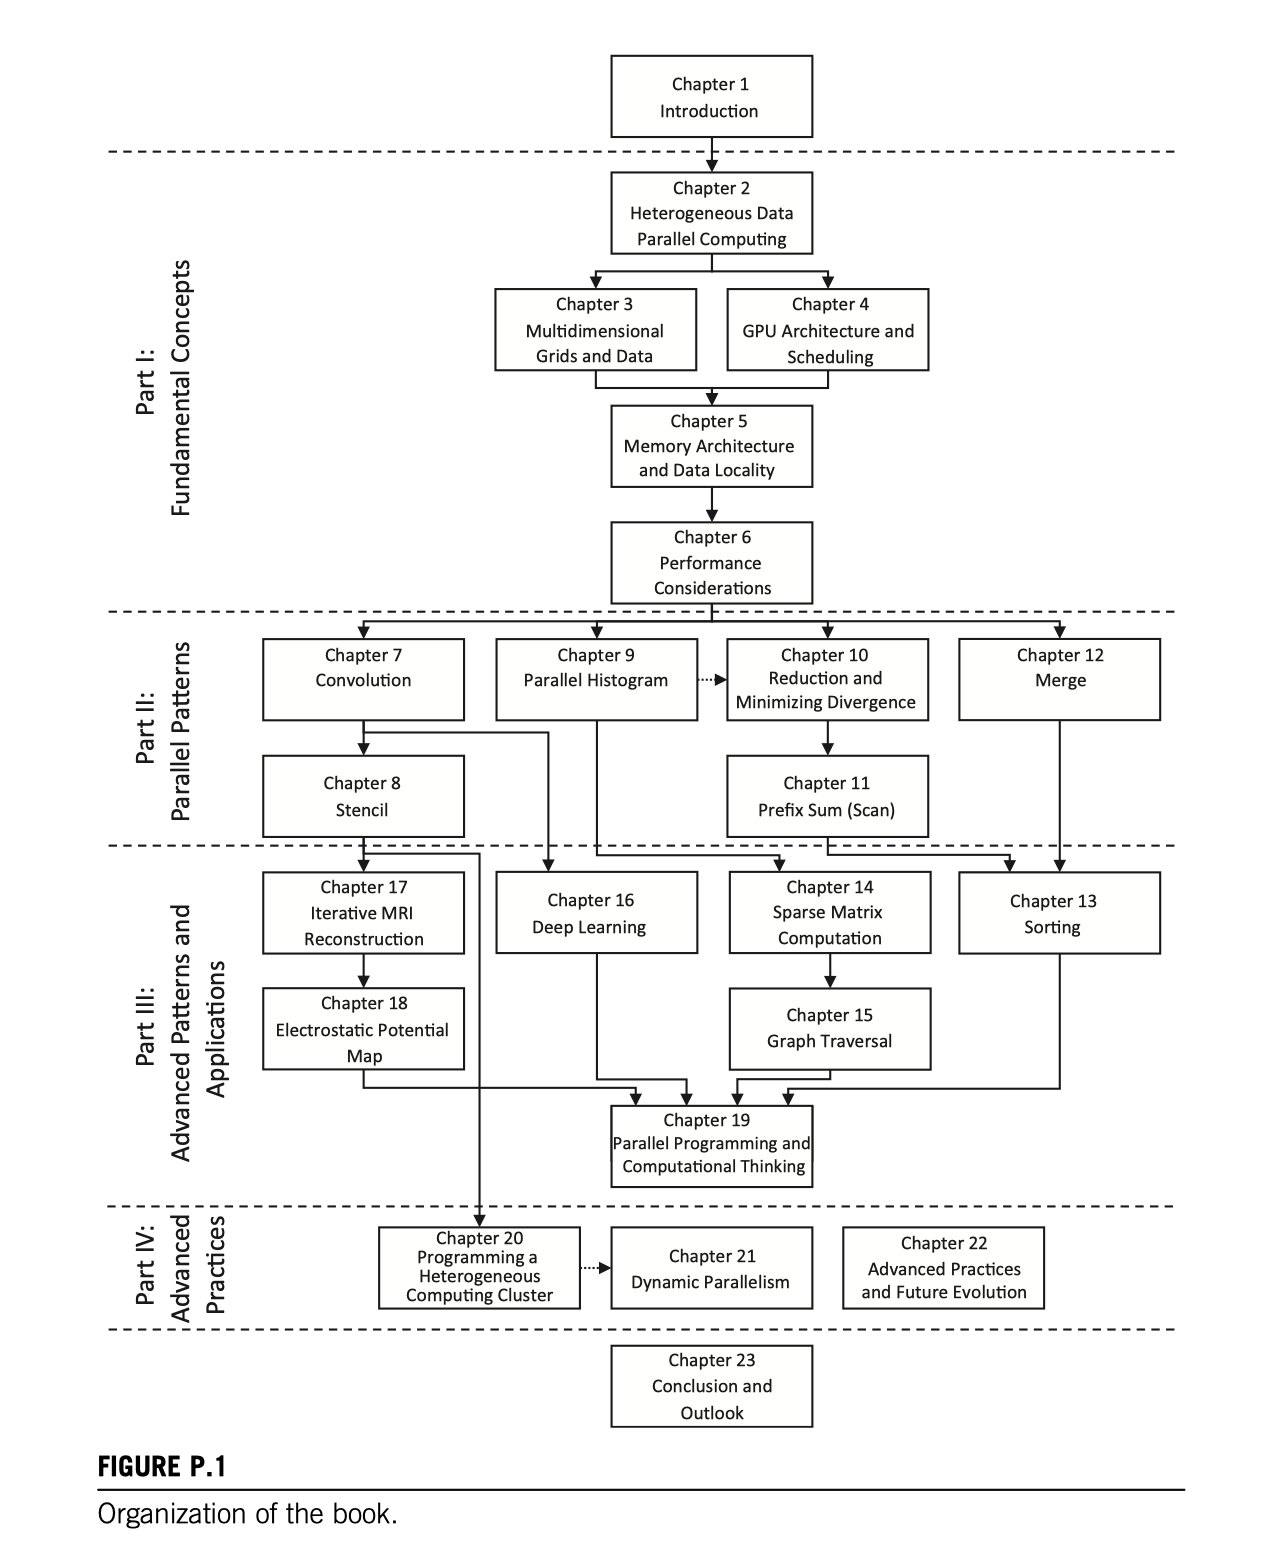
\includegraphics[width=\textwidth]{figs/P.1.png}
\end{figure}

\subsection{如何使用这本书}
我们希望通过本书提供一些教学课程的经验。 自 2006 年以来,我们教授多种类型的课程:一学期课程和一周强化课程。 
最初的 ECE498AL 课程已成为伊利诺伊大学香槟分校的永久课程,称为 ECE408 或 CS483。 
当我们第二次提供 ECE498AL 时,我们开始编写本书的一些早期章节。 
前四章也在 Nicolas Pinto 于 2009 年春天教授的麻省理工学院课程中进行了测试。
从那时起,我们将这本书用于 ECE408 的众多课程以及 Coursera 异构并行编程课程以及 VSCSE 和 PUMPS 暑期学校 。

\subsection{两阶段方法}
书中的大部分章节都设计为每节大约 75 分钟的讲座。 可能需要两节 75 分钟的讲座才能完全讲完的章节
是第 11 章(前缀和(扫描))、第 14 章(稀疏矩阵计算)和第 15 章(图遍历)。 
在 ECE408 中,讲座、编程作业和期末项目是同步进行的,并分为两个阶段。

在第一阶段,即本书的第一部分和第二部分,学生学习基础知识和基本模式,并练习通过指导性编程作业所学到的技能。 
此阶段由 12 章组成,通常需要大约 7 周的时间。 每周,学生都会完成与该周讲座相对应的编程作业。 
例如,第一周,基于第2章的讲座专门讲授基本的CUDA内存/线程模型、CUDA对C语言的扩展以及基本的编程工具。 
讲座结束后,学生可以在几个小时内编写简单的向量加法代码。

接下来的两周包括基于第 3 章到第 6 章的一系列四堂讲座,让学生对 CUDA 内存模型、CUDA 线程执行模型、
GPU 硬件性能特征和现代计算机系统架构有概念性的理解。 
在这两周内,学生们研究矩阵-矩阵乘法的不同实现,他们会看到在此期间其实现的性能如何显着提高。 
在剩下的四个星期中,讲座涵盖了基于第 7 章到第 12 章开发高性能并行应用程序所需的常见数据并行编程模式。
在这几周中,学生完成有关卷积、直方图、约简和前缀和的作业。 在第一阶段结束时,学生应该对并行编程非常熟悉,
并且应该准备好以更少的操作来实现更高级的代码。

在第二阶段(由第三部分和第四部分组成)中,学生在完成涉及加速高级模式或应用程序的最终项目时学习高级模式和应用程序。 
他们还学习了在完成项目时可能会发现有用的高级实践。 尽管我们通常不会在此阶段分配每周的编程作业,
但该项目通常有一个每周里程碑来帮助学生调整自己的节奏。 根据课程的持续时间和形式,教师可能无法涵盖此阶段的所有章节,
可能需要跳过一些章节。 教师还可以选择用客座讲座、论文讨论会或支持最终项目的讲座来代替一些讲座。 
因此,图 P.1 使用箭头来指示章节之间的依赖关系,以帮助教师选择可以跳过或重新排序的章节,以根据其特定上下文定制课程。

\subsection{将它们结合在一起:最终项目}
虽然本书的讲座、实验和章节有助于为学生奠定知识基础,但将学习经验整合在一起的是最终项目。 
最终项目对于整个学期的课程非常重要,因此它在课程中占据显着位置,需要近两个月的时间来重点关注。 
它包含五个创新方面:指导、研讨会、临床、最终报告和研讨会。 
虽然有关最终项目的大部分信息都可以在伊利诺伊州 NVIDIA GPU 教学套件中找到,但我们仍想提供这些方面设计背后的推理。

鼓励学生将他们的最终项目基于代表研究界当前挑战的问题。 为了推动这一过程,
教师应该招募几个计算科学研究小组来提出问题并担任导师。 导师被要求提供一份一到两页的项目规格表,
简要描述申请的重要性、导师希望与学生团队一起完成申请的目标、技术技能(特定类型的数学、物理) 和化学课程),
这是理解和使用应用程序所需的,以及学生可以利用的网络和传统资源列表,以获取技术背景、一般信息和构建块,
以及特定实现的特定 URL 或 FTP 路径 和编码示例。 
这些项目规格表还为学生提供了在其职业生涯后期定义自己的研究项目的学习经验。 
伊利诺伊州-NVIDIA GPU 教学套件中提供了几个示例。

\subsection{设计文档}
一旦学生决定了一个项目并组建了一个团队,他们就需要提交该项目的设计文件。 
这有助于他们在投入项目之前仔细考虑项目步骤。 进行此类规划的能力对于他们以后的职业成功非常重要。 
设计文件应讨论项目的背景和动机、应用程序级目标和潜在影响、最终应用程序的主要特征、
设计概述、实施计划、性能目标、验证计划和验收测试 ,以及项目进度表。

\subsection{项目报告及座谈会}
学生需要提交一份关于其团队主要发现的项目报告。 我们还建议举办全天的班级研讨会。 
在研讨会期间,学生使用与团队规模成比例的演示时段。 
在演示过程中,学生们为了全班同学的利益而突出了他们的项目报告中最好的部分。 
演讲占学生成绩的很大一部分。 每个学生必须单独回答针对该学生的问题,因此可以为同一团队中的个人分配不同的成绩。 
研讨会为学生提供了一个学习如何进行简洁演示的机会,以激励他们的同伴阅读全文。

\subsection{班级竞赛}
2016年ECE408的招生规模远远超过了最终项目进程所能容纳的水平。 结果,我们从期末项目变成了班级竞赛。 
在学期中期,我们宣布了一个竞赛挑战问题。 我们用一个讲座来解释比赛挑战问题以及用于对团队进行排名的规则。 
所有学生提交的内容都会自动评分和排名。 每个团队的最终排名取决于其并行代码的执行时间、正确性和清晰度。 
学生在学期结束时演示他们的解决方案并提交最终报告。 当班级规模导致最终项目不可行时,这种妥协保留了最终项目的一些好处。

\subsection{课程资源}
伊利诺伊州-NVIDIA GPU 教学套件是一个公开资源,其中包含讲座幻灯片和录音、实验作业、
最终项目指南以及为在课堂上使用本书的教师提供的示例项目规范。 此外,我们正在公开基于本书的伊利诺伊州本科生和研究生课程。 
虽然本书为这些课程提供了知识内容,但附加材料对于实现总体教育目标至关重要。

最后,我们鼓励您提交反馈。 如果您有任何改进本书的想法,我们希望收到您的来信。 我们想知道如何改进在线补充材料。 
当然,我们也想知道您喜欢这本书的哪些方面。 我们期待您的回音。


\newpage
\section{介绍}

自从计算出现以来,许多高价值应用程序都需要比计算设备所能提供的更高的执行速度和资源。 
早期应用依靠处理器速度、内存速度和内存容量的进步来增强应用级能力,如天气预报的及时性、工程结构分析的准确性、
计算机生成图形的真实性、航班预订数量等 每秒处理的资金转账数量。 
最近,深度学习等新应用程序需要比最好的计算设备所能提供的更多的执行速度和资源。 
这些应用需求在过去五年中推动了计算设备功能的快速进步,并且在可预见的未来将继续如此。

基于单个中央处理单元 (CPU) 的微处理器似乎按顺序步骤执行指令,例如 Intel 和 AMD 的 x86 处理器中的微处理器,
配备快速增加的时钟频率和硬件资源,推动了20世纪80年代和90年代的计算机应用性能的快速提高和成本的降低。 
在二十年的发展过程中,这些单 CPU 微处理器为桌面带来了 GFLOPS,即每秒千兆 ($10^9$) 次浮点运算,为数据中心带来了 TFLOPS,
即每秒万亿 ($10^{12}$) 次浮点运算。 这种对性能改进的不懈追求使得应用软件能够提供更多功能、
拥有更好的用户界面并生成更有用的结果。 反过来,一旦用户习惯了这些改进,他们就会要求更多的改进,
从而为计算机行业创造一个积极(良性)的循环。

然而,自 2003 年以来,由于能源消耗和散热问题,这种正向驱动的速度已经放缓。 
这些问题限制了时钟频率的增加以及单个 CPU 内每个时钟周期内可以执行的生产活动,同时保持了按顺序步骤执行指令的外观。 
从那时起,几乎所有微处理器供应商都转向了在每个芯片中使用多个物理 CPU(称为处理器内核)的模型,以提高处理能力。 
在这个模型中,传统的CPU可以被视为单核CPU。 为了受益于多个处理器内核,用户必须拥有多个指令序列,
无论是来自相同应用程序还是不同应用程序,都可以在这些处理器内核上同时执行。 对于要从多个处理器核心中受益的特定应用程序,
其工作必须分为可以在这些处理器核心上同时执行的多个指令序列。 
从单 CPU 按顺序执行指令到多核并行执行多个指令序列的转变对软件开发人员社区产生了巨大影响。

传统上,绝大多数软件应用程序都是作为顺序程序编写的,由处理器执行,
这些处理器的设计是冯·诺依曼在 1945 年的开创性报告中设想的(冯·诺依曼等人,1972 年)。 
人们可以将这些程序的执行理解为基于程序计数器(在文献中也称为指令指针)的概念按顺序单步执行代码。 
程序计数器包含处理器将执行的下一条指令的内存地址。 由应用程序的这种顺序、
逐步执行产生的指令执行活动序列在文献中被称为执行线程,或简称为线程。 线程的概念非常重要,
因此本书的其余部分将对其进行更正式的定义和广泛的使用。

从历史上看,大多数软件开发人员依赖硬件的进步,例如提高时钟速度和在后台执行多条指令,来提高顺序应用程序的速度; 
随着每一代新处理器的推出,相同的软件运行得更快。 计算机用户也越来越期望这些程序在每一代新一代微处理器上运行得更快。 
这种期望十多年来一直不成立。 顺序程序将仅在一个处理器内核上运行,一代又一代不会变得明显更快。 
如果没有性能改进,随着新微处理器的推出,应用程序开发人员将无法再在其软件中引入新的特性和功能; 
这减少了整个计算机行业的增长机会。

相反,每一代新一代微处理器将继续享受显着性能改进的应用软件将是并行程序,其中多个执行线程协作以更快地完成工作。 
并行程序相对于顺序程序的这种新的、显着提升的优势被称为并发革命(Sutter 和 Larus,2005)。 
并行编程的实践绝不是新鲜事。 几十年来,高性能计算 (HPC) 社区一直在开发并行程序。 
这些并行程序通常在昂贵的大型计算机上运行。 只有少数精英应用程序可以证明使用这些计算机是合理的,
从而将并行编程的实践限制在少数应用程序开发人员中。 现在所有新的微处理器都是并行计算机,
需要开发为并行程序的应用程序数量急剧增加。 现在软件开发人员非常需要学习并行编程,这也是本书的重点。

\subsection{异构并行计算}
自 2003 年以来,半导体行业已经确定了微处理器设计的两条主要轨迹(Hwu 等人,2008 年)。 
多核轨迹旨在在进入多核的同时保持顺序程序的执行速度。 多核始于两核处理器,并且核心数量随着每一代半导体工艺的发展而增加。 
最近的一个例子是最新的 Intel 多核服务器微处理器,具有多达 24 个处理器核心,每个处理器核心都是无序、多指令发布处理器,
实现完整的 x86 指令集,支持具有两个硬件线程的超线程,旨在最大限度地提高性能。 顺序程序的执行速度。 
另一个例子是最新的 ARM Ampere 多核服务器处理器,具有 128 个处理器内核。

相比之下,多线程轨迹更关注并行应用程序的执行吞吐量。 多线程轨迹始于大量线程,并且线程数量再次随着每一代的增加而增加。 
最近的一个例子是 NVIDIA Tesla A100 图形处理单元 (GPU),它具有数万个线程,在大量简单、有序的管道中执行。 
自 2003 年以来,多线程处理器,尤其是 GPU,一直在浮点性能竞赛中处于领先地位。
截至 2021 年,A100 GPU 的峰值浮点吞吐量为 64 位双精度 9.7 TFLOPS,32 位单精度 156 TFLOPS,
16 位半精度为 312 TFLOPS。 相比之下,最新的英特尔 24 核处理器的双精度峰值浮点吞吐量为 0.33 TLOPS,
单精度为 0.66 TFLOPS。 过去几年,多线程 GPU 和多核 CPU 之间的峰值浮点计算吞吐量之比一直在增加。 
这些不一定是应用程序速度; 它们只是这些芯片中执行资源可以支持的原始速度。

多核和多线程之间的峰值性能之间如此巨大的差距已经形成了显着的“电势”积累,在某些时候,必须做出一些让步。 
我们已经达到了这一点。 迄今为止,这种巨大的峰值性能差距已经促使许多应用程序开发人员将其软件的计算密集型部分转移到 
GPU 上执行。 也许更重要的是,并行执行性能的大幅提升使得革命性的新应用成为可能,例如本质上由计算密集型部分组成的深度学习。 
毫不奇怪,这些计算密集型部分也是并行编程的主要目标:当有更多工作要做时,
就有更多机会在协作的并行工作线程(即线程)之间分配工作。

{\color{red} Fig 1.1}

有人可能会问,为什么多线程 GPU 和多核 CPU 之间的峰值性能差距如此之大。 答案在于两种类型处理器之间基本设计理念的差异,
如图 1.1 所示。 如图 1.1A 所示,CPU 的设计针对顺序代码性能进行了优化。 
算术单元和操作数数据传送逻辑的设计旨在最大限度地减少算术运算的有效延迟,但代价是增加芯片面积和每单元功耗的使用。 
大型末级片上高速缓存旨在捕获频繁访问的数据,并将一些长延迟内存访问转换为短延迟高速缓存访问。 
复杂的分支预测逻辑和执行控制逻辑用于减轻条件分支指令的延迟。 通过减少操作的延迟,CPU 硬件减少了每个单独线程的执行延迟。 
然而,低延迟算术单元、复杂的操作数传送逻辑、大型高速缓冲存储器和控制逻辑消耗了芯片面积和功率,
否则这些芯片面积和功率可用于提供更多算术执行单元和存储器访问通道。 这种设计方法通常称为面向延迟的设计。

另一方面,GPU 的设计理念是由快速发展的视频游戏行业塑造的,
该行业对在高级游戏中执行大量浮点计算和每帧内存访问的能力提出了巨大的经济压力。 
这种需求促使 GPU 供应商寻找方法来最大化专用于浮点计算和内存访问吞吐量的芯片面积和功率预算。

在图形应用程序中,每秒执行大量浮点计算以完成视点变换和对象渲染等任务是非常直观的。 
此外,每秒执行大量内存访问的需求同样重要,甚至可能更重要。 
许多图形应用程序的速度受到数据从内存系统传送到处理器的速率的限制,反之亦然。 
GPU 必须能够将大量数据移入和移出其 DRAM(动态随机存取存储器)中的图形帧缓冲区,
因为这种移动可以使视频显示丰富并满足游戏玩家的需求。 
游戏应用程序普遍接受的宽松内存模型(各种系统软件、应用程序和 I/O 设备期望其内存访问工作的方式)
也使 GPU 更容易支持访问内存的大规模并行性。

相比之下,通用处理器必须满足传统操作系统、应用程序和 I/O 设备的要求,这些要求对支持并行内存访问提出了更多挑战,
从而使提高内存访问(通常称为内存)的吞吐量,常被称为内存带宽,变得更加困难。 
因此,图形芯片的运行内存带宽大约是同时可用 CPU 芯片的 10 倍,我们预计 GPU 在内存带宽方面将在一段时间内继续保持优势。

一个重要的观察是,就功耗和芯片面积而言,减少延迟比增加吞吐量要昂贵得多。 
例如,可以通过将运算单元的数量加倍来使运算吞吐量加倍,但代价是芯片面积和功耗加倍。 
然而,将算术延迟减少一半可能需要将电流加倍,但代价是所用芯片面积增加一倍以上,功耗增加四倍。 
因此,GPU 的主流解决方案是优化大量线程的执行吞吐量,而不是减少单个线程的延迟。 
这种设计方法允许流水线内存通道和算术运算具有较长的延迟,从而节省了芯片面积和功耗。 
内存访问硬件和算术单元的面积和功率的减少使得 GPU 设计者可以在芯片上拥有更多的硬件和算术单元,从而提高总执行吞吐量。 
图 1.1 通过在图 1.1A 的 CPU 设计中显示较少数量的较大算术单元和较少数量的内存通道,直观地说明了设计方法的差异,
与图 1.1B 中大量的较小算术单元和大量的存储器通道形成对比。

这些 GPU 的应用软件预计将使用大量并行线程编写。 当其中一些线程等待长延迟内存访问或算术运算时,
硬件会利用大量线程来寻找要做的工作。 图 1.1B 中的小型高速缓冲存储器用于帮助控制这些应用程序的带宽需求,
以便访问相同内存数据的多个线程不需要全部访问 DRAM。 这种设计风格通常称为面向吞吐量的设计,
因为它力求最大化大量线程的总执行吞吐量,同时允许单个线程可能需要更长的执行时间。

应该清楚的是,GPU 被设计为并行的、面向吞吐量的计算引擎,它们在某些 CPU 设计为能很好执行的任务上表现不佳。 
对于只有一个或很少线程的程序,具有较低操作延迟的CPU可以获得比GPU高得多的性能。 
当程序有大量线程时,具有较高执行吞吐量的GPU可以获得比CPU高得多的性能。 
因此,我们应该预料到许多应用程序会同时使用 CPU 和 GPU,在 CPU 上执行顺序部分,在 GPU 上执行数值密集型部分。 
这就是 NVIDIA 于 2007 年推出的统一计算设备架构 (CUDA) 编程模型旨在支持应用程序的 CPU-GPU 联合执行的原因。

还需要注意的是,当应用程序开发人员选择运行其应用程序的处理器时,速度并不是唯一的决定因素。 其他几个因素可能更为重要。 
首先也是最重要的是,所选处理器必须在市场上占有很大的份额,称为处理器的安装基础。 原因很简单。 
大量的客户群最能证明软件开发成本的合理性。 在市场份额较小的处理器上运行的应用程序不会有大量的客户群。 
这一直是传统并行计算系统的一个主要问题,与通用微处理器相比,传统并行计算系统的市场份额可以忽略不计。 
只有少数由政府和大公司资助的精英应用程序在这些传统的并行计算系统上成功开发。 多线程 GPU 改变了这种情况。 
由于 GPU 在 PC 市场的受欢迎,其销量已达数亿。 几乎所有台式电脑和高端笔记本电脑都配备了 GPU。 
迄今为止,已使用超过 10 亿个支持 CUDA 的 GPU。 如此庞大的市场占有率使这些 GPU 对应用程序开发人员来说具有经济吸引力。

另一个重要的决定因素是实用的外形因素和易于访问性。 直到 2006 年,并行软件应用程序都在数据中心服务器或部门集群上运行。 
但这样的执行环境往往会限制这些应用程序的使用。 比如在医学影像这样的应用中,发表一篇基于64节点集群机的论文就可以了。 
但磁共振成像 (MRI) 机器的实际临床应用是基于 PC 和特殊硬件加速器的某种组合。 
原因很简单,GE 和西门子等制造商无法在临床环境中销售需要计算机服务器机架的 MRI,而这在学术部门环境中很常见。 
事实上,美国国立卫生研究院 (NIH) 在一段时间内拒绝资助并行编程项目; 他们认为并行软件的影响将是有限的,
因为基于集群的大型机器无法在临床环境中工作。 如今,许多公司都配备了 GPU 的 MRI 产品,
美国国立卫生研究院 (NIH) 也资助使用 GPU 计算的研究。

直到 2006 年,图形芯片都非常难以使用,因为程序员必须使用相当于图形 API(应用程序编程接口)功能来访问处理单元,
这意味着需要 OpenGL 或 Direct3D 技术来对这些芯片进行编程。 更简单地说,计算必须表示为以某种方式绘制像素的函数,
以便在这些早期的 GPU 上执行。 该技术称为 GPGPU,用于使用 GPU 进行通用编程。 即使使用更高级别的编程环境,
底层代码仍然需要适合用于绘制像素的 API。 这些 API 限制了人们实际上可以为早期 GPU 编写的应用程序类型。 
因此,GPGPU 并没有成为一种广泛的编程现象。 尽管如此,这项技术还是足够令人兴奋,激发了一些英勇的努力和出色的研究成果。

2007 年,随着 CUDA 的发布,一切都发生了变化(NVIDIA,2007)。 CUDA 并不单独代表软件变更; 
芯片中添加了额外的硬件。 NVIDIA实际上专门投入了硅片面积以方便并行编程。 在 G80 及其后续并行计算芯片中,
GPGPU 程序根本不再通过图形接口。 相反,硅芯片上的新通用并行编程接口可以满足 CUDA 程序的要求。 
通用编程接口极大地扩展了可以轻松为 GPU 开发的应用程序类型。 所有其他软件层也都重新设计,
以便程序员可以使用熟悉的 C/C++ 编程工具。

虽然 GPU 是异构并行计算中的一类重要计算设备,但还有其他重要类型的计算设备在异构计算系统中用作加速器。 
例如,现场可编程门阵列已被广泛用于加速网络应用。 本书中介绍的使用 GPU 作为学习工具的技术也适用于这些加速器的编程任务。

\subsection{为什么要提高速度或并行性?}
正如我们在 1.1 节中所述,大规模并行编程的主要动机是让应用程序在未来的硬件世代中享受持续的速度提升。 
正如我们将在并行模式、高级模式和应用程序(第二部分和第三部分,第 7 章到第 19 章)中讨论的那样,
当应用程序适合并行执行时,在 GPU 上良好的实现可以比在单个 CPU 内核上顺序执行获得 100 倍以上的加速。
如果应用程序包含我们所说的“数据并行性”,通常只需几个小时的工作即可实现 10x 的加速。

人们可能会问为什么应用程序将继续要求提高速度。 我们今天拥有的许多应用程序似乎运行得足够快。 
尽管当今世界有无数的计算应用程序,但未来许多令人兴奋的大众市场应用程序都是我们之前认为的超级计算应用程序或超级应用程序。 
例如,生物学研究界正在越来越多地进入分子水平。 显微镜可以说是分子生物学中最重要的仪器,过去依赖光学或电子仪器。 
然而,我们使用这些仪器进行的分子水平观察存在局限性。 通过结合计算模型来模拟具有传统仪器设置的边界条件的基础分子活动,
可以有效地解决这些限制。 通过模拟,我们可以测量更多的细节并测试更多的假设,这比仅使用传统仪器所能想象的要多。 
在可预见的未来,就可建模的生物系统的规模以及可在可容忍响应时间内模拟的反应时间长度而言,这些模拟将继续受益于计算速度的提高。 
这些增强将对科学和医学产生巨大影响。

对于视频和音频编码和操作等应用,请考虑与旧式 NTSC 电视相比,我们对数字高清 (HD) 电视的满意度。 
一旦我们在高清电视上体验到图像的细节水平,就很难再回到旧技术了。 但请考虑高清电视所需的所有处理。 
这是一个高度并行的过程,三维 (3D) 成像和可视化也是如此。 
未来,视图合成和低分辨率视频的高分辨率显示等新功能将需要电视具有更高的计算能力。 
在消费者层面,我们将开始看到越来越多的视频和图像处理应用程序,这些应用程序可以改善图片和视频的焦点、光照和其他关键方面。

更高的计算速度带来的好处之一是更好的用户界面。 智能手机用户现在可以享受到与大屏幕电视相媲美的高分辨率触摸屏的更自然的界面。 
毫无疑问,这些设备的未来版本将整合具有 3D 视角的传感器和显示器、
结合虚拟和物理空间信息以增强可用性的应用程序以及基于语音和计算机视觉的界面,从而需要更高的计算速度。

消费电子游戏领域也正在进行类似的发展。 过去,在游戏中驾驶汽车只是一组预先安排好的场景。 
如果你的车撞到了障碍物,你的车的路线不会改变; 只是游戏比分发生了变化。 您的车轮没有弯曲或损坏,即使您失去了一个车轮,
驾驶也不再困难。 随着计算速度的提高,游戏可以基于动态模拟而不是预先安排的场景。 
我们可以期待在未来体验到更多这样的现实效果。 事故会损坏你的车轮,你的在线驾驶体验将会更加真实。 
精确建模物理现象的能力已经激发了数字孪生的概念,其中物理对象在模拟空间中具有精确的模型,
从而可以以更低的成本彻底进行压力测试和恶化预测。 众所周知,物理效应的真实建模和模拟需要非常大量的计算能力。

通过大幅提高计算吞吐量而实现的新应用程序的一个重要例子是基于人工神经网络的深度学习。 
虽然神经网络自 20 世纪 70 年代以来一直在积极研究,但它们在实际应用中一直无效,
因为训练这些网络需要太多的标记数据和太多的计算。 互联网的兴起提供了大量带标签的图片,GPU 的兴起带来了计算吞吐量的激增。 
因此,自 2012 年以来,基于神经网络的应用在计算机视觉和自然语言处理领域得到了快速采用。
这种采用彻底改变了计算机视觉和自然语言处理应用,并引发了自动驾驶汽车和家庭辅助设备的快速发展。

我们提到的所有新应用程序都涉及以不同方式和在不同级别模拟和/或表示物理并发世界,并处理大量数据。 
有了如此大量的数据,大部分计算可以在数据的不同部分上并行完成,尽管它们必须在某些时候进行协调。 
在大多数情况下,数据交付的有效管理会对并行应用程序的可实现速度产生重大影响。 
虽然这样做的技术通常为一些每天使用此类应用程序的专家所熟知,
但绝大多数应用程序开发人员可以从对这些技术的更直观的理解和实际工作知识中受益。

我们的目标是以直观的方式向应用程序开发人员展示数据管理技术,这些开发人员的正规教育可能不是计算机科学或计算机工程。 
我们还旨在提供许多实用的代码示例和实践练习,帮助读者获取工作知识,
这需要一个实用的编程模型来促进并行实现并支持数据交付的正确管理。 CUDA 提供了这样的编程模型,
并且已经过大型开发者社区的充分测试。

\subsection{加速实际的应用}
通过并行化应用程序,我们可以期望获得多少加速? 计算系统 A 相对于计算系统 B 的应用程序加速比的定义是,
在系统 B 中执行应用程序所用的时间与在系统 A 中执行相同应用程序所用的时间之比。
例如,如果应用程序在系统 A 中执行需要花费 10 秒,而在系统 B 中执行需要 200 秒,
则系统 A 相对于系统 B 的执行加速为 200/10=20,称为 20x(20 倍)加速。

并行计算系统相对于串行计算系统可实现的加速取决于可以并行化的应用程序部分。 
例如,如果可并行部分所花费的时间百分比为 30\%,则并行部分加速 100x 将使应用程序的总执行时间减少不超过 29.7\%。 
也就是说,整个应用程序的加速大约仅为 1/(1 - 0.297)=1.42x。 事实上,即使在并行部分进行无限量的加速,
也只能将执行时间减少 30\%,实现的加速不超过 1.433。 
通过并行执行可以实现的加速水平可能会受到应用程序的可并行部分的严重限制,这一事实被称为阿姆达尔定律(Amdahl,2013)。 
另一方面,如果 99\% 的执行时间都在并行部分,则并行部分加速 100x 会将应用程序执行时间减少到原始时间的 1.99\%。 
这使整个应用程序加速了 50x。 因此,对于大规模并行处理器来说,应用程序的绝大多数执行都在并行部分进行,
以有效加快其执行速度,这一点非常重要。

研究人员已在某些应用程序中实现了超过 100x 的加速。 然而,这通常只有在算法得到增强后进行大量优化和调整才能实现,
这样超过 99.9\% 的应用程序工作都在并行部分。

应用程序可实现的加速水平的另一个重要因素是从内存访问和写入数据的速度。 在实践中,
应用程序的直接并行化通常会导致内存 (DRAM) 带宽饱和,从而仅带来大约 10x 的加速。 诀窍在于找出如何解决内存带宽限制,
这涉及到进行多种转换之一,以利用专门的 GPU 片上内存来大幅减少对 DRAM 的访问次数。 
然而,必须进一步优化代码以克服片上内存容量有限等限制。 本书的一个重要目标是帮助读者充分理解这些优化并熟练使用它们。

请记住,单核 CPU 执行所实现的加速水平也可以反映 CPU 对应用程序的适用性。 在某些应用程序中,CPU 的性能非常好,
这使得使用 GPU 加速性能变得更加困难。 大多数应用程序都有一些可以由 CPU 更好地执行的部分。 
我们必须给CPU一个公平的执行机会,并确保编写的代码能够让GPU补充CPU的执行,
从而正确地利用CPU/GPU组合系统的异构并行计算能力。 
截至目前,结合了多核 CPU 和众核 GPU 的大众市场计算系统已经为笔记本电脑带来了万亿级计算,为集群带来了百亿亿级计算。

{\color{red} Fig 1.2}

图 1.2 说明了典型应用的主要部分。 实际应用程序的大部分代码往往是连续的。 这些连续的部分被图示为桃子的“核”区域; 
尝试将并行计算技术应用于这些部分就像咬桃核一样——感觉不太好! 这些部分很难并行化。 CPU 在这些部分往往做得非常好。 
好消息是,虽然这些部分可能占用大部分代码,但它们往往只占超级应用程序执行时间的一小部分。

然后是我们所说的“桃肉”部分。 这些部分很容易并行化,一些早期的图形应用程序也是如此。 
异构计算系统中的并行编程可以极大地提高这些应用程序的速度。 如图1.2所示,早期的GPGPU编程接口只覆盖了桃肉部分的一小部分,
这类似于最令人兴奋的应用程序的一小部分。 正如我们将看到的,CUDA 编程接口旨在涵盖令人兴奋的应用程序的更大部分。 
并行编程模型及其底层硬件仍在快速发展,以实现更大的应用程序部分的高效并行化。

\subsection{并行编程中的挑战}
是什么让并行编程变得困难? 有人曾经说过,如果不关心性能,并行编程是很容易的。 您实际上可以在一小时内编写一个并行程序。 
但是,如果您不关心性能,为什么还要编写并行程序呢?

本书解决了在并行编程中实现高性能的几个挑战。 首先,设计具有与顺序算法相同的算法(计算)复杂度的并行算法可能具有挑战性。 
许多并行算法执行与顺序算法相同的工作量。 然而,一些并行算法比顺序算法做更多的工作。 事实上,有时他们可能会做太多的工作,
以至于最终在大型输入数据集上运行速度变慢。 这尤其是一个问题,因为快速处理大型输入数据集是并行编程的重要动机。

例如,许多现实世界的问题最自然地用数学递归来描述。 并行化这些问题通常需要以非直观的方式思考问题,
并且可能需要在执行过程中进行冗余工作。 有一些重要的算法原语,例如前缀和,可以促进将问题的顺序递归公式转换为更并行的形式。 
我们将更正式地介绍工作效率的概念,并将说明设计并行算法所涉及的方法和权衡,
这些算法可以使用重要的并行模式(例如第 11 章“前缀”中的前缀和)实现与顺序算法相同水平的计算复杂性 总和(扫描)。

其次,许多应用程序的执行速度受到内存访问延迟和/或吞吐量的限制。 我们将这些应用程序称为内存限制应用程序; 
相比之下,计算密集型应用程序受到每字节数据执行的指令数量的限制。 
在内存受限的应用程序中实现高性能并行执行通常需要提高内存访问速度的方法。 
我们将在第 5 章“内存架构和数据局部性”和第 6 章“性能注意事项”中介绍内存访问的优化技术,
并将在有关并行模式和应用程序的几个章节中应用这些技术。

第三,并行程序的执行速度通常比顺序程序的情况对输入数据特征更敏感。 许多现实世界的应用程序需要处理具有广泛变化特征的输入,
例如不稳定或不可预测的数据大小以及不均匀的数据分布。 这些大小和分布的变化可能会导致分配给并行线程的工作量不均匀,
并可能显着降低并行执行的效率。 并行程序的性能有时会因这些特征而发生巨大变化。 
我们将在介绍并行模式和应用程序的章节中介绍用于规范数据分布和/或动态细化线程数量的技术,以应对这些挑战。

第四,某些应用程序可以并行化,同时几乎不需要跨不同线程进行协作。 这些应用程序通常被称为“令人尴尬的并行”。 
其他应用程序需要线程相互协作,这需要使用同步操作,例如屏障或原子操作。 这些同步操作给应用程序带来了开销,
因为线程经常会发现自己在等待其他线程而不是执行有用的工作。 我们将在本书中讨论减少同步开销的各种策略。

幸运的是,研究人员已经解决了大部分挑战。 跨应用程序域还存在一些常见模式,
使我们能够将在一个域中派生的解决方案应用于其他域中的挑战。 
这是我们将在重要的并行计算模式和应用程序的背景下提出解决这些挑战的关键技术的主要原因。

\subsection{相关并行编程接口}
在过去的几十年里,人们提出了许多并行编程语言和模型(Mattson 等,2004)。 
最广泛使用的是用于共享内存多处理器系统的 OpenMP(Open,2005)和用于可扩展集群计算的消息传递接口(MPI)(MPI,2009)。 
两者都已成为主要计算机供应商支持的标准化编程接口。

OpenMP 实现由编译器和运行时组成。 程序员向 OpenMP 编译器指定有关循环的指令(命令)和编译指示(提示)。 
通过这些指令和编译指示,OpenMP 编译器可以生成并行代码。 运行时系统通过管理并行线程和资源来支持并行代码的执行。 
OpenMP 最初是为 CPU 执行而设计的,现已扩展为支持 GPU 执行。 OpenMP 的主要优点是它提供编译器自动化和运行时支持,
以从程序员那里抽象出许多并行编程细节。 
这种自动化和抽象有助于使应用程序代码在不同供应商生产的系统以及同一供应商的不同代系统之间更加可移植。 
我们将此属性称为性能可移植性。 然而,在 OpenMP 中进行有效的编程仍然需要程序员了解所涉及的所有详细的并行编程概念。 
由于 CUDA 为程序员提供了对这些并行编程细节的明确控制,因此即使对于那些想要使用 OpenMP 作为主要编程接口的人来说,
它也是一种极好的学习工具。 此外,根据我们的经验,OpenMP 编译器仍在不断发展和改进。 
许多程序员可能需要使用 CUDA 风格的接口来处理 OpenMP 编译器无法满足的部分。

另一方面,MPI 是一种编程接口,其中集群中的计算节点不共享内存(MPI,2009)。 
所有的数据共享和交互都必须通过显式的消息传递来完成。 MPI在HPC中得到了广泛的应用。 
用MPI编写的应用程序已在超过10万个节点的集群计算系统上成功运行。 如今,许多 HPC 集群都采用异构 CPU/GPU 节点。 
由于计算节点之间缺乏共享内存,将应用程序移植到 MPI 所需的工作量可能相当大。 
程序员需要执行域分解以跨各个节点划分输入和输出数据。 在域分解的基础上,
程序员还需要调用消息发送和接收函数来管理节点之间的数据交换。 相比之下,
CUDA 为 GPU 中的并行执行提供共享内存来解决这一难题。 虽然 CUDA 是与每个节点的有效接口,
但大多数应用程序开发人员需要使用 MPI 在集群级别进行编程。 
此外,通过 NVIDIA Collective Communications Library (NCCL) 等 API,CUDA 中的多 GPU 编程支持不断增加。 
因此,HPC 中的并行程序员了解如何在使用多 GPU 节点的现代计算集群中进行联合 MPI/CUDA 编程非常重要,
该主题将在第 20 章“异构计算集群编程”中介绍。

2009 年,包括 Apple、Intel、AMD/ATI 和 NVIDIA 在内的几家主要行业参与者联合开发了一种名为
开放计算语言 (OpenCL) 的标准化编程模型(The Khronos Group,2009)。 与 CUDA 类似,
OpenCL 编程模型定义了语言扩展和运行时 API,以允许程序员管理大规模并行处理器中的并行性和数据交付。 
与 CUDA 相比,OpenCL 更多地依赖 API,更少地依赖语言扩展。 
这使得供应商能够快速调整其现有的编译器和工具来处理 OpenCL 程序。 OpenCL 是一种标准化的编程模型,
用 OpenCL 开发的应用程序无需修改即可在所有支持 OpenCL 语言扩展和 API 的处理器上正确运行。 
然而,人们可能需要修改应用程序才能实现新处理器的高性能。

熟悉 OpenCL 和 CUDA 的人都知道,OpenCL 和 CUDA 的关键概念和功能之间存在显着的相似性。 
也就是说,CUDA程序员可以以最小的努力学习OpenCL编程。 更重要的是,
几乎所有在使用 CUDA 中学到的技术都可以轻松应用于 OpenCL 编程。

\subsection{总体目标}
我们的主要目标是教读者如何对大规模并行处理器进行编程以实现高性能。 
因此,本书的大部分内容都致力于开发高性能并行代码的技术。 我们的方法不需要大量的硬件专业知识。 
然而,您需要对并行硬件架构有一个很好的概念性理解,以便能够推断代码的性能行为。 
因此,我们将用一些篇幅来直观地理解基本的硬件架构特性,并用许多篇幅来介绍开发高性能并行程序的技术。 
特别是,我们将重点关注计算思维(Wing,2006)技术,这些技术将使您能够以适合大规模并行处理器上高性能执行的方式思考问题。

大多数处理器上的高性能并行编程需要了解硬件的工作原理。 可能需要很多年才能构建工具和机器,
使程序员能够在没有这些知识的情况下开发高性能代码。 即使我们有这样的工具,
我们怀疑了解硬件知识的程序员将能够比那些不了解硬件的程序员更有效地使用这些工具。 
因此,我们专门用第 4 章“计算架构和调度”来介绍 GPU 架构的基础知识。 
作为高性能并行编程技术讨论的一部分,我们还讨论了更专业的体系结构概念。

我们的第二个目标是教授并行编程的正确功能和可靠性,这是并行计算中的一个微妙问题。 
过去从事并行系统工作的程序员都知道,仅实现初始性能是不够的。 挑战在于以一种可以调试代码并支持用户的方式来实现它。 
CUDA 编程模型鼓励使用简单形式的屏障同步、内存一致性和原子性来管理并行性。 
此外,它还提供了一系列强大的工具,使人们不仅可以调试功能方面,还可以调试性能瓶颈。 
我们将证明,通过关注数据并行性,可以在应用程序中实现高性能和高可靠性。

我们的第三个目标是通过探索并行编程方法来实现未来硬件各代的可扩展性,
以便未来的机器(将越来越并行)可以比今天的机器更快地运行代码。 我们希望帮助您掌握并行编程,
以便您的程序可以扩展到新一代机器的性能水平。 这种可扩展性的关键是规范和本地化内存数据访问,
以最大限度地减少关键资源的消耗和更新数据结构时的冲突。 
因此,开发高性能并行代码的技术对于确保应用程序未来的可扩展性也很重要。

实现这些目标需要大量的技术知识,因此我们将在本书中介绍并行编程的相当多的原理和模式(Mattson et al., 2004)。 
我们不会单独教授这些原则和模式。 我们将在并行化有用应用程序的背景下教授他们。 
然而,我们无法涵盖所有这些技术,因此我们选择了最有用且经过充分验证的技术来详细介绍。 
事实上,当前版本有关并行模式的章节数量显着增加。 现在我们准备向您提供本书其余部分的快速概述。

\subsection{本书的组织}
本书分为四个部分。 第一部分涵盖并行编程、数据并行、GPU 和性能优化的基本概念。 
这些基础章节为读者提供了成为 GPU 程序员所需的基本知识和技能。 第二部分介绍了原始并行模式,
第三部分介绍了更高级的并行模式和应用程序。 这两部分应用了第一部分中学到的知识和技能,
并根据需要介绍了其他 GPU 架构特性和优化技术。 最后一部分(第四部分)介绍了高级实践,
以帮助想要成为专家 GPU 程序员的读者完善知识。

关于基本概念的第一部分由第 2 章至第 6 章组成。 第 2 章,异构数据并行计算,介绍数据并行性和 CUDA C 编程。 
本章依赖于读者之前具有 C 编程经验的事实。 它首先介绍了 CUDA C 作为 C 的简单、小型扩展,
支持异构 CPU/GPU 计算和广泛使用的单程序、多数据并行编程模型。 
然后,它涵盖了以下方面所涉及的思维过程:(1) 识别要并行化的应用程序部分,
(2) 隔离并行化代码要使用的数据,使用 API 函数在并行计算设备上分配内存, (3)使用API函数将数据传输到并行计算设备,
(4)将并行部分开发为将由并行线程执行的内核函数,(5)启动由并行线程执行的内核函数,
以及( 6) 最终通过 API 函数调用将数据传输回主机处理器。 我们使用向量加法的运行示例来说明这些概念。 
虽然本章的目标是教授 CUDA C 编程模型的足够概念,以便读者能够编写简单的并行 CUDA C 程序,
但它涵盖了开发基于任何并行编程接口的并行应用程序所需的几种基本技能。

第 3 章“多维网格和数据”介绍了 CUDA 并行执行模型的更多细节,特别是它涉及使用线程的多维组织处理多维数据。 
它对线程的创建、组织、资源绑定和数据绑定提供了足够的洞察力,使读者能够使用 CUDA C 实现复杂的计算。

第 4 章,计算架构和调度,介绍 GPU 架构,重点介绍如何组织计算核心以及如何调度线程在这些核心上执行。 
讨论了各种架构注意事项,以及它们对 GPU 架构上执行的代码性能的影响。 其中包括透明可扩展性、SIMD 执行和控制发散、
多线程和延迟容忍以及占用等概念,所有这些都在本章中进行了定义和讨论。

第 5 章“内存架构和数据局部性”通过讨论 GPU 的内存架构来扩展第 4 章“计算架构和调度”。 
它还讨论了可用于保存 CUDA 变量以管理数据传输和提高程序执行速度的特殊存储器。 
我们介绍分配和使用这些内存的 CUDA 语言功能。 适当地使用这些存储器可以极大地提高数据访问吞吐量,
并有助于缓解存储器系统中的流量拥塞。

第 6 章“性能注意事项”介绍了当前 CUDA 硬件中的几个重要的性能注意事项。 
特别是,它提供了有关所需的线程执行和内存访问模式的更多详细信息。 
这些细节构成了程序员推理其组织计算和数据决策的后果的概念基础。 
本章最后列出了 GPU 程序员经常用来优化任何计算模式的常见优化策略清单。 
该清单将在本书的接下来的两部分中使用,以优化各种并行模式和应用程序。

关于原始并行模式的第二部分由第 7 章至第 12 章组成。 第 7 章“卷积”介绍了卷积,这是一种常用的并行计算模式,
植根于数字信号处理和计算机视觉,需要仔细管理数据访问局部性。 我们还使用这种模式在现代 GPU 中引入恒定内存和缓存。 
第 8 章“模板”介绍了模板,这是一种类似于卷积的模式,但植根于求解微分方程,
并且具有为进一步优化数据访问局部性提供独特机会的特定功能。 我们还使用此模式来介绍线程和数据的 3D 组织,
并展示第 6 章“性能注意事项”中介绍的针对线程粒度的优化。

第 9 章“并行直方图”介绍了直方图,这是一种广泛用于统计数据分析以及大型数据集中的模式识别的模式。 
我们还使用这种模式引入原子操作作为协调共享数据并发更新和私有化优化的手段,从而减少了这些操作的开销。 
第 10 章“归约和最小化分支”介绍了归约树模式,该模式用于总结输入数据的集合。 
我们还使用此模式来演示控制分支发散对性能的影响,并展示如何减轻这种影响的技术。 
第 11 章“前缀和(扫描)”介绍了前缀和或扫描,这是一种重要的并行计算模式,它将固有的顺序计算转换为并行计算。 
我们还使用这种模式来引入并行算法中工作效率的概念。 最后,第 12 章“合并”介绍了并行合并,
这是一种在分而治之工作分区策略中广泛使用的模式。 我们还用本章来介绍动态输入数据的识别和组织。

关于高级并行模式和应用程序的第三部分在精神上与第二部分类似,但所涵盖的模式更详细,并且通常包含更多应用程序上下文。 
因此,这些章节不太关注介绍新技术或功能,而是更关注特定于应用程序的注意事项。 对于每个应用程序,
我们首先确定制定并行执行基本结构的替代方法,然后推理每个替代方案的优点和缺点。 
然后,我们完成实现高性能所需的代码转换步骤。 这些章节帮助读者将前面章节中的所有材料放在一起,
并在他们承担自己的应用程序开发项目时为他们提供支持。

第三部分由第 13 章至第 19 章组成。 第 13 章“排序”介绍了并行排序的两种形式:基数排序和合并排序。 
这种高级模式利用了前面章节中介绍的更原始的模式,特别是前缀和和并行合并。 第 14 章,稀疏矩阵计算,介绍了稀疏矩阵计算,
它广泛用于处理非常大的数据集。 本章向读者介绍了重新排列数据以实现更有效的并行访问的概念:数据压缩、填充、排序、转置
和正则化。 第 15 章,图遍历,介绍图算法以及如何在 GPU 编程中有效地实现图搜索。 提出了许多不同的并行图算法策略,
并讨论了图结构对最佳算法选择的影响。 这些策略建立在更原始的模式之上,例如直方图和合并。

第 16 章“深度学习”涵盖了深度学习,它正在成为 GPU 计算的一个极其重要的领域。 我们介绍了卷积神经网络的有效实现,
并将更深入的讨论留给其他来源。 卷积神经网络的高效实现利用了平铺等技术和卷积等模式。 第 17 章,迭代磁共振成像重建,
涵盖非笛卡尔 MRI 重建以及如何利用循环融合和分散-聚集变换等技术来增强并行性并减少同步开销。 第 18 章,静电势图,
涵盖了分子可视化和分析,这得益于通过应用稀疏矩阵计算中的经验教训来处理不规则数据的技术。

第 19 章“并行编程和计算思维”介绍了计算思维,即以更适合 HPC 的方式制定和解决计算问题的艺术。 
它通过涵盖组织程序的计算任务以使它们可以并行完成的概念来实现这一点。 我们首先讨论将抽象的科学、
特定问题的概念组织成计算任务的转化过程,这是生产高质量串行或并行应用软件的重要的第一步。 
然后本章讨论并行算法结构及其对应用程序性能的影响,这是基于 CUDA 性能调优经验。 
尽管我们没有深入探讨这些替代并行编程风格的实现细节,
但我们希望读者能够利用在本书中获得的基础来学习其中任何一种编程风格的编程。 
我们还提出了一个高级案例研究,以展示通过创造性计算思维可以看到的机会。

第四部分高级实践由第 20 至 22 章组成。 第 20 章,异构计算集群编程,介绍了异构集群上的 CUDA 编程,
其中每个计算节点都由 CPU 和 GPU 组成。 
我们讨论使用 MPI 和 CUDA 来集成节点间计算和节点内计算以及由此产生的通信问题和实践。 
第 21 章“CUDA 动态并行性”介绍了动态并行性,即 GPU 根据数据或程序结构动态为自身创建工作的能力,
而不是总是等待 CPU 这样做。 第 22 章“高级实践和未来发展”列出了 CUDA 程序员需要了解的重要的各种高级功能和实践。 
其中包括零复制内存、统一虚拟内存、多个内核同时执行、函数调用、异常处理、调试、分析、双精度支持、
可配置缓存/暂存器大小等主题。 例如,早期版本的 CUDA 在 CPU 和 GPU 之间提供有限的共享内存功能。 
程序员需要显式管理 CPU 和 GPU 之间的数据传输。 然而,当前版本的 CUDA 支持统一虚拟内存和零拷贝内存等功能,
可实现 CPU 和 GPU 之间的数据无缝共享。 有了这样的支持,CUDA 程序员可以将变量和数据结构声明为在 CPU 和 GPU 之间共享。 
运行时硬件和软件保持一致性,并根据需要自动代表程序员执行优化的数据传输操作。 
这种支持显着降低了与计算和 I/O 活动重叠的数据传输所涉及的编程复杂性。 在教科书的介绍部分,
我们使用 API 进行显式数据传输,以便读者更好地了解幕后发生的情况。 
我们稍后会在第 22 章“高级实践和未来演进”中介绍统一虚拟内存和零拷贝内存。

虽然本书中的章节都是基于 CUDA 的,但它们总体上帮助读者建立了并行编程的基础。 
我们相信,当我们从具体的例子中学习时,人类能够最好地理解。 也就是说,我们必须首先在特定编程模型的上下文中学习概念,
这为我们将知识推广到其他编程模型时提供了坚实的基础。 当我们这样做时,我们可以从 CUDA 示例中汲取具体经验。 
对CUDA的深入体验也使我们变得成熟,这将有助于我们学习甚至可能与CUDA模型无关的概念。

第 23 章“结论和展望”提供了结论性意见以及对大规模并行编程的未来的展望。 我们首先重新审视我们的目标,
并总结各章如何组合在一起以帮助实现目标。 最后,我们预测大规模并行计算的快速进步将使其成为未来十年最令人兴奋的领域之一。


\end{document}


























